In order to assess the influence of interface conditions on the outgassing flux, simulations are performed with chemical potential continuity (Equation \ref{eq: c/s conservation}) or mobile concentration continuity assuming in both cases flux conservation (Equation \ref{eq: flux conservation}).
For the sake of simplicity and to emphasis on the influence of interface conditions, no trapping was assumed and ideal Dirichlet boundary conditions were set.
Simulations were performed on two test cases: W/Cu and Cu/EUROFER.
The materials properties used for the simulations can be found in Table \ref{tab:materials properties_1}.
In both cases the solute concentration $c_\mathrm{m}$ was set to \SI{1e20}{m^{-3}} at $x=0$ and zero on the other boundary.

% The governing equations for the diffusion problem with conservation of chemical potential read:
% \begin{subequations}
%     \begin{align}
%         \frac{\partial c_\mathrm{m}}{\partial t} &=\nabla \cdot\left(D(T) \nabla c_\mathrm{m}\right) \\
%         D^- \nabla c_\mathrm{m}^- &= D^+ \nabla c_\mathrm{m}^+ \\
%         \left(\frac{c_\mathrm{m}}{S}\right)^- &= \left(\frac{c_\mathrm{m}}{S}\right)^+
%     \end{align}
% \end{subequations}
% where $c_\mathrm{m}$ is the concentration of mobile H in \si{m^{-3}}, $D$ is the diffusion coefficient in \si{m^2.s^{-1}}, $S$ is the solubility of H in the material in \si{m^{-3}.Pa^{-0.5}}.
% The exponents $+$ and $-$ denote the two sides of the interface between the two subdomains.

% not necessary...
% \subsection{W/Cu case}
% A \SI{4}{mm}-thick slab made of \SI{2}{mm} of W (referred as $\Omega_1$) and \SI{2}{mm} of Cu (referred as $\Omega_2$)  at $T=\SI{500}{K}$ was first simulated.


% \begin{figure*}
%     \centering
%     \subfloat[Solute profiles at steady state (W/Cu)]{%
%         \label{fig: solute profiles w cu}
%         \begin{overpic}[width=0.5\linewidth]{Figures/Chapter3/monoblocks/interface_condition/w_cu/solute_profiles.pdf}
%             \put(35, 55){W}
%             \put(65, 35){Cu}
%         \end{overpic}
%     }
%     \subfloat[Outgassing flux (W/Cu)]{%
%         \label{fig: outgassing flux w cu}
%         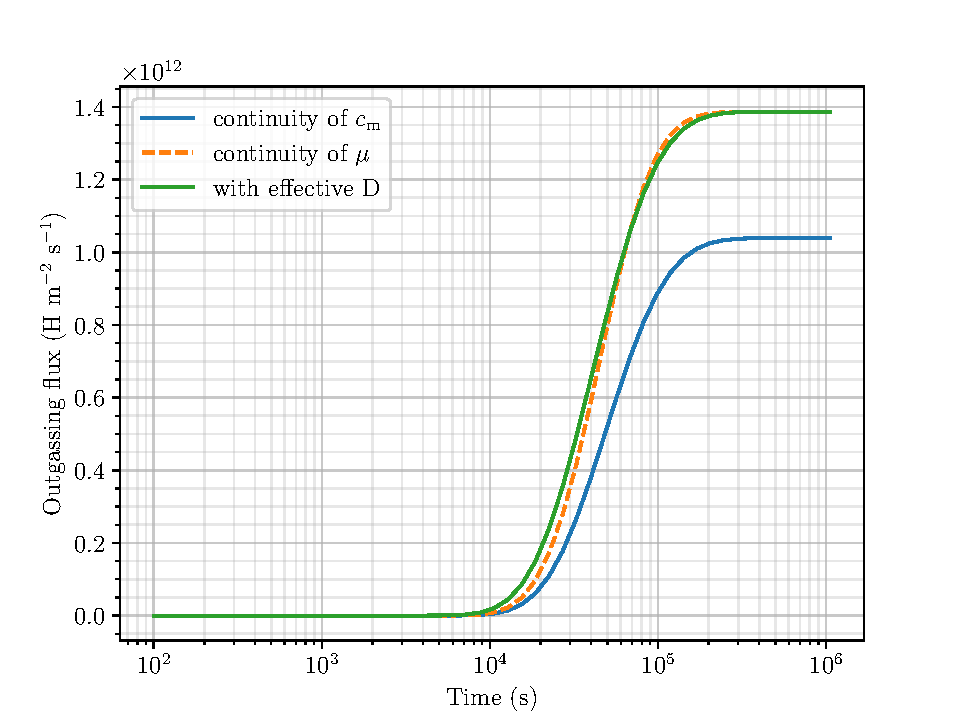
\includegraphics[width=0.5\linewidth]{Figures/Chapter3/monoblocks/interface_condition/w_cu/comparison_fluxes.pdf}
%     } \\
%     \subfloat[Solute profiles at steady state (Cu/EUROFER)]{%
%         \label{fig: solute profiles cu eurofer}
%         \begin{overpic}[width=0.5\linewidth]{Figures/Chapter3/monoblocks/interface_condition/cu_eurofer/solute_profiles_cu_eurofer.pdf}
%             \put(35, 55){Cu}
%             \put(65, 35){EUROFER}
%         \end{overpic}
%      }
%     \subfloat[Outgassing flux (Cu/EUROFER)]{%
%         \label{fig: outgassing flux cu eurofer}
%         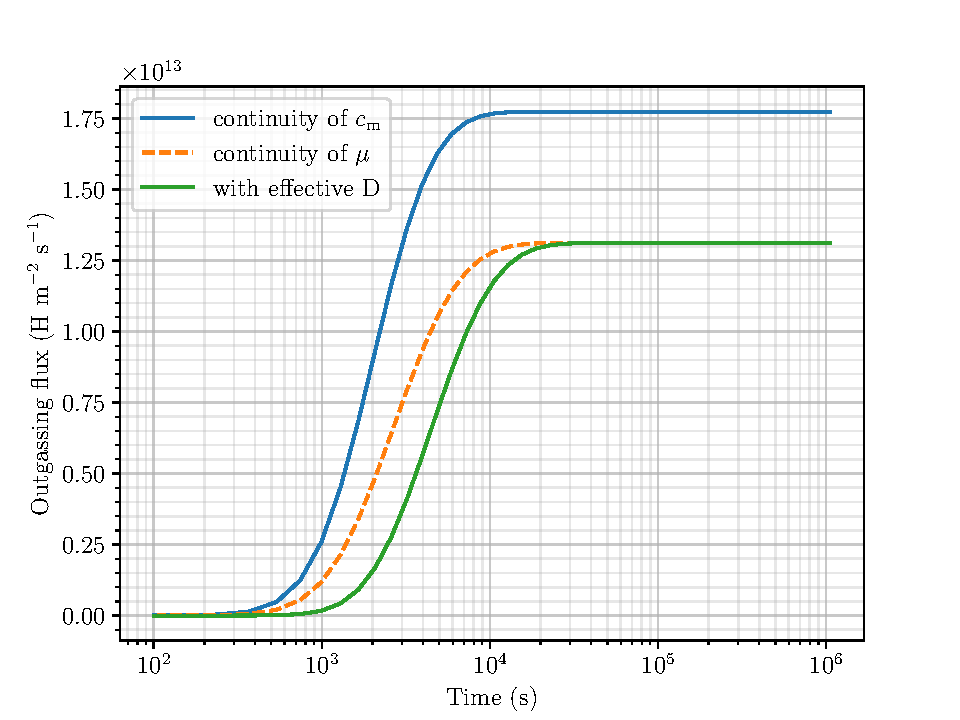
\includegraphics[width=0.5\linewidth]{Figures/Chapter3/monoblocks/interface_condition/cu_eurofer/comparison_fluxes_cu_eurofer.pdf}
%      }
%     \caption{Influence of chemical potential conservation}
%     \label{fig: influence of mu bi material}
% \end{figure*}

% In this case, the conservation of chemical potential resulted in higher steady-state concentration gradients (see Figure \ref{fig: solute profiles w cu}) due to the higher solubility of Cu.
% For a given temperature (and therefore given diffusion coefficients), this implied an increase of the outgassing flux (see Figure \ref{fig: outgassing flux w cu}) compared to the case with concentration continuity.

% \subsection{Cu/EUROFER case}

% A \SI{4}{mm}-thick slab made of \SI{2}{mm} of Cu (referred as $\Omega_1$) and \SI{2}{mm} of EUROFER (referred as $\Omega_2$) at $T=\SI{600}{K}$ was simulated.
% Since the solubility of EUROFER is lower than that of Cu, the steady-state concentration gradients (see Figure \ref{fig: solute profiles cu eurofer}) were lower compared to the case with concentration continuity.
% The outgassing flux was therefore lower in the case of chemical potential conservation (see Figure \ref{fig: outgassing flux cu eurofer}).

% \subsection{Identification technique}
% Assuming the diffusion coefficients are known, the solubility coefficients in both materials can be identified by determining an effective diffusion coefficient.

% The steady-state flux $\varphi_\infty$ can be expressed from Equations \ref{eq:MES c} and \ref{eq: MES c coefficients} as follow:
% \begin{subequations}
%     \begin{align}
%         \varphi_\infty &= -D_2 \nabla c_2 =  -D_1 \nabla c_1 \\
%         &= -D_2 a_2 \frac{c_\mathrm{m}(x=0)}{L} = -D_1 a_1 \frac{c_\mathrm{m}(x=0)}{L}\\
%         &= -a_0 D_\mathrm{eq} \frac{c_\mathrm{m}(x=0)}{L}
%     \end{align}
%     \label{eq: steady state flux 1}
% \end{subequations}
% where the indexes $1$ and $2$ denote the left and right subdomains respectively and $L$ is the size of the domain in total.

% If this method allows to measure solubilities, it is however not always convenient considering the time required to reach steady-state.
% One way to overcome this difficulty is to compute an equivalent effective diffusion coefficient noted $D_\mathrm{eff}$.
% $D_\mathrm{eff}$ is computed by assuming an homogeneous material and a linear steady state profile.
% The steady-state flux can therefore be written as:
% \begin{subequations}
%     \begin{align}
%         \varphi_\infty &= -D_\mathrm{eff} \nabla c \\
%         &= -D_\mathrm{eff} \frac{c_\mathrm{m}(x=L) - c_\mathrm{m}(x=0)}{L} \\
%     \end{align}
%     \label{eq: steady state flux 2}
% \end{subequations}

% By combining Equations \ref{eq: steady state flux 1} and \ref{eq: steady state flux 2}, $D_\mathrm{eff}$ reads:
% \begin{equation}
%     D_\mathrm{eff} = \frac{a_0 \; D_\mathrm{eq} \; c_\mathrm{m}(x=0) }{c_\mathrm{m}(x=L) - c_\mathrm{m}(x=0)}
% \end{equation}

% By fitting measurements of the outgassing flux with either an analytical transient solution or a simulation code (see Figures \ref{fig: outgassing flux w cu} and \ref{fig: outgassing flux cu eurofer}), one can estimate $D_\mathrm{eff}$ and therefore the coefficient $a_0$ which can finally be correlated to material properties (see Equation \ref{eq: MES c coefficients}).

% However, some discrepancies were found between this method and the actual outgassing curve during the transient phase.
% One way of getting rid of these is to fit the curve with an analytical solution of transient mass transfer in a 1D composite slab with conservation of chemical potential.
% This can be utterly complex and is well beyond the scope of this study.

% Moreover, surface effects and the presence of traps often complicate the analysis of the experimental data.
% Therefore, a more thorough identification technique would be to use embedded hydrogen transport codes such as FESTIM in a parametric optimisation algorithm as described in previous work \sidecite{delaporte-mathurin_parametric_2021}.
% Such a process could be able to determine materials properties such as diffusion coefficients, solubilities and trap densities.

\subsection{Methodology}
\subsubsection{Geometry}
The 2D geometry is defined on Figure \ref{fig: monoblock 2d geometry}.

\begin{figure}
    %  \subfloat[1D geometry \label{fig: monoblock 1D geometry}]{%
    %     \begin{overpic}[width=0.5\linewidth]{Figures/Chapter3/monoblocks/interface_condition/iter case/Monoblock 1D.pdf}
    %         \put(40, 50){\SI{6}{mm}}
    %         \put(40, 8){W}
    %         \put(62, 50){\SI{1}{mm}}
    %         \put(65, 8){Cu}
    %         \put(72, 50){\SI{1.5}{mm}}
    %         \put(72, 8){CuCrZr}
    %         \put(6, 25){\large$\Gamma_\mathrm{top}$}
    %         \put(85, 25){\large$\Gamma_\mathrm{coolant}$}
    %     \end{overpic}
    %  }
     \subfloat[2D geometry]{%
        \begin{overpic}[width=\linewidth]{Figures/Chapter3/monoblocks/interface_condition/iter case/monoblock_sketch.pdf}
            \put(42, 5){\SI{28}{mm}}
            \put(97, 50){\SI{28}{mm}}
            \put(10, 32){\SI{13.5}{mm}}
            \put(42, 62){ \diameter \SI{12}{mm}}
            \put(42, 71){ \diameter \SI{15}{mm}}
            \put(42, 76){ \diameter \SI{17}{mm}}
            \put(20, 80){\large$\Gamma_\mathrm{top}$}
            \put(4, 60){\large$\Gamma_\mathrm{lateral}$}
            \put(78, 60){\large$\Gamma_\mathrm{lateral}$}
            \put(40, 41){\large$\Gamma_\mathrm{coolant}$}
        \end{overpic}
     }
     \caption{2D ITER monoblock geometry showing W armour \cruleme[grey]{0.3cm}{0.3cm}, Cu interlayer \cruleme[orange]{0.3cm}{0.3cm}, CuCrZr alloy cooling pipe  \cruleme[yellow]{0.3cm}{0.3cm}}\label{fig: monoblock geometry}
     \label{fig: monoblock 2d geometry}
    \end{figure}

\subsubsection{Materials properties}
The materials properties that have been set are detailed in Table \ref{tab:materials properties_1} and their thermal dependency is shown on Figure \ref{fig:properties_1}.
The trap properties in each material are detailed in Table \ref{tab:traps monoblock_1}.
All traps are homogeneously distributed in the materials, except for Trap 2 which is only located in the first micrometre behind the plasma facing surface $\Gamma_\mathrm{top}$ (see Figure \ref{fig: monoblock geometry}) to account for damage creation.

\begin{table*}
    \centering
    \begin{tabular}{p{1.7cm}  R{3cm}  R{3cm}  R{1.8cm}  R{1cm} R{1.8cm}  R{1cm}}
         & \multicolumn{2}{c}{Thermal properties} & \multicolumn{4}{c}{Hydrogen transport properties}\\
        \hline
        Material & $\rho \cdot C_p \newline(\si{J.K^{-1}.m^{-3}})$ & $\lambda \newline(\si{W.m^{-1}.K^{-1}})$ & $D_0 \newline(\si{m^2.s^{-1}})$ & $E_\mathrm{diff} \newline(\si{eV})$ & $S_0 \newline(\si{m^{-3}.Pa^{-0.5}})$ & $E_\mathrm{S} \newline(\si{eV})$\\
        \hline
        \\
        W \cite{frauenfelder_solution_1969}& %
        $5.1\times 10^{-6} \cdot T^3 \newline - 8.3\times 10^{-2}\cdot T^2 \newline + 6.0 \times 10^{2}\cdot T \newline +2.4\times 10^6$ &%
        $-7.8\times 10^{-9}\cdot T^3 \newline %
        +5.0\times 10^{-5}\cdot T^2 \newline%
        -1.1\times 10^{-1} \cdot T \newline%
        +1.8\times 10^{2}$ &%
        $2.4\times 10^{-7}$ & 0.39 &%
        $1.87\times 10^{24}$ & 1.04\\
        \\
        Cu \cite{reiter_compilation_1996}&%
        $1.7\times 10^{-4}\cdot T^3\newline %
        +6.1\times 10^{-2}\cdot T^2\newline %
        +4.7\times 10^2\cdot T\newline %
        +3.5\times 10^6$ &%

        $-3.9\times 10^{-8}\cdot T^3\newline %
        +3.8\times 10^{-5}\cdot T^2\newline %
        -7.9\times 10^{-2}\cdot T\newline %
        +4.0\times 10^2 $&%

        $6.6\times 10^{-7}$ &%
        0.39&%
        $3.14\times 10^{24}$ & 0.57\\
        \\
        CuCrZr \cite{serra_hydrogen_1998}& %
        $-1.8\times 10^{-4}\cdot T^3 \newline %
        +1.5\times 10^{-1}\cdot T^2\newline %
        +6.2\times 10^2\cdot T\newline %
        +3.5\times 10^6$ &%

        $5.3\times 10^{-7}\cdot T^3\newline %
        -6.5\times 10^{-4}\cdot T^2\newline %
        +2.6\times 10^{-1}\cdot T\newline %
        +3.1\times 10^2$ & %

        $3.9\times 10^{-7}$ & %
        0.42&%
        $4.28\times 10^{23}$ & 0.39\\
        \\
        EUROFER \cite{aiello_hydrogen_2002} & %
        - & - &
        $1.5\times 10^{-7}$ & %
        0.15 & %
        $6.14\times 10^{20}$ & 0.25
        \\
        \\
    \end{tabular}
    \caption{Materials properties used in the simulations. Thermal properties are fitted from ANSYS.}
    \label{tab:materials properties_1}
\end{table*}

\begin{figure}
    \centering
    \begin{subfigure}{\linewidth}
        \centering
        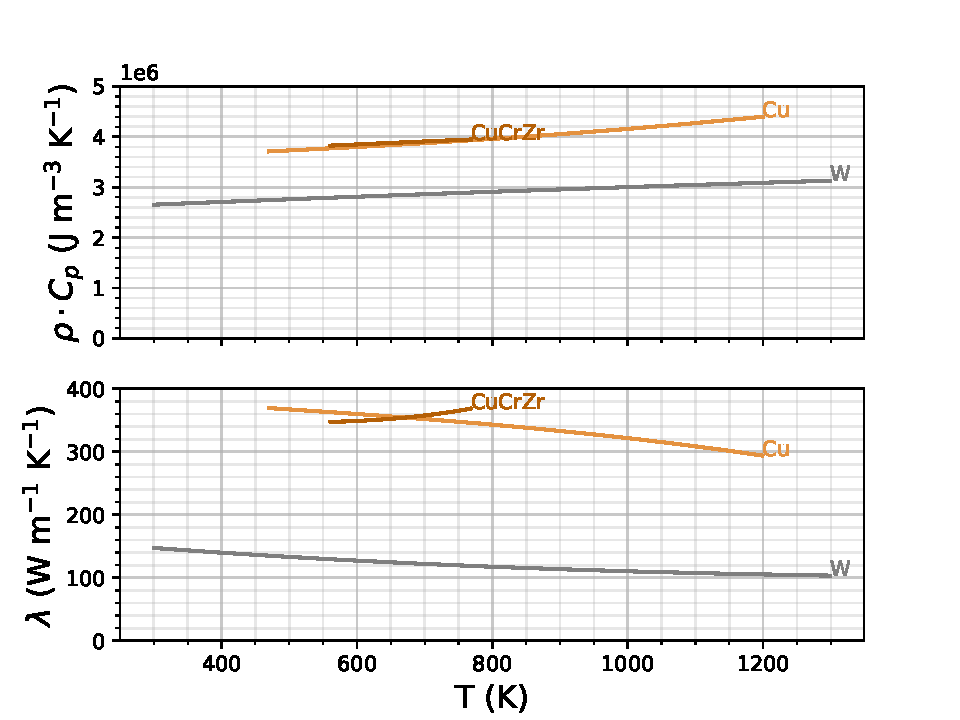
\includegraphics[width=\linewidth]{Figures/Chapter3/monoblocks/interface_condition/iter case/thermal_prop.pdf}
        \caption{Thermal properties}
    \end{subfigure}
    \begin{subfigure}{\linewidth}
        \centering
        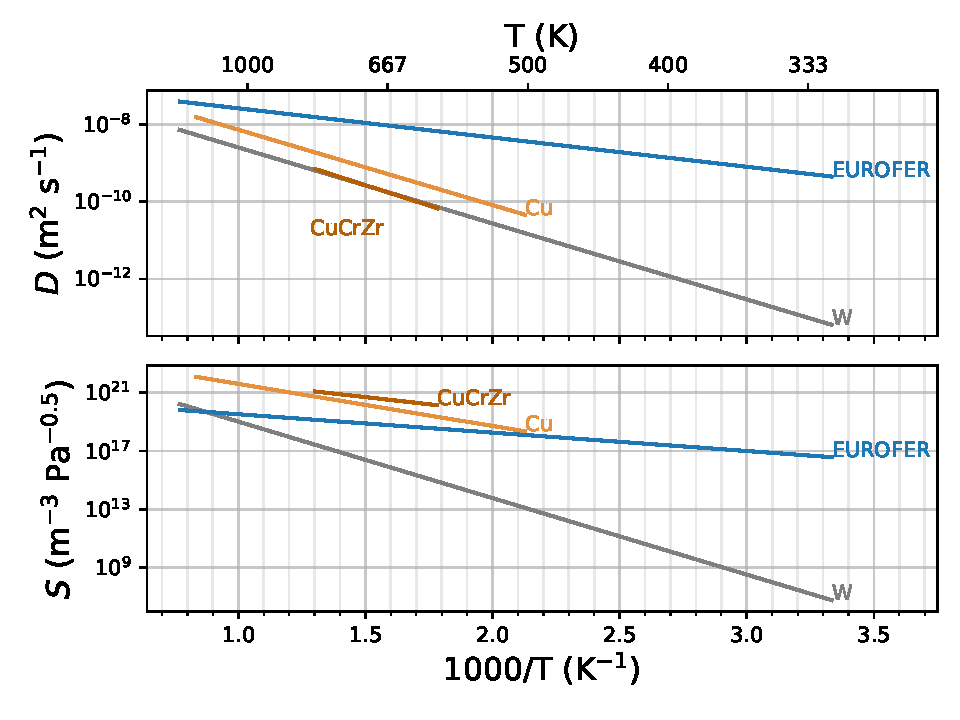
\includegraphics[width=\linewidth]{Figures/Chapter3/monoblocks/interface_condition/H_properties.pdf}
        \caption{H transport properties}
    \end{subfigure}
    \caption{Material properties used in the simulations \cite{frauenfelder_solution_1969, reiter_compilation_1996, serra_hydrogen_1998, aiello_hydrogen_2002}}
    \label{fig:properties_1}
\end{figure}

\begin{table*}
    \centering
    \begin{tabular}{L{1.5cm} L{1.5cm} R{1.6cm} R{1.1cm} R{1.6cm} R{1.1cm} R{2cm}}
         & Material & $k_0 (\si{m^3.s^{-1}})$ &  $E_k (\si{eV})$ & $p_0 (\si{s^{-1}})$ & $E_p (\si{eV})$ & $n_i (\si{at.fr.})$ \\
        \hline
        \\
        Trap 1 & W & $3.8 \times 10^{-17}$ & 0.39 & $8.4 \times 10^{12}$& 1.20 & $5.0 \times 10^{-4}$ \\
        \\
       Trap 2 & W & $3.8 \times 10^{-17}$ & 0.39 & $8.4 \times 10^{12}$& 1.40 & $5.0 \times 10^{-3}$ \\
        \\
        Trap 3 & Cu & $6.0 \times 10^{-17}$ & 0.39 & $8.0 \times 10^{13}$ & 0.50 &$5.0 \times 10^{-5}$\\
        \\
        Trap 4 & CuCrZr & $1.2\times 10^{-16}$ & 0.42 & $8.0 \times 10^{13}$ & 0.50 &$5.0 \times 10^{-5}$\\
        \\
        Trap 5 & CuCrZr & $1.2\times 10^{-16}$ & 0.42 & $8.0 \times 10^{13}$ & 0.83 &$4.0 \times 10^{-2}$\\
        \\
    \end{tabular}
    \caption{Traps properties used in the simulations \cite{hodille_macroscopic_2015, dolan_assessment_1994}}
    \label{tab:traps monoblock_1}
\end{table*}


\subsubsection{Boundary conditions}
The source term $\varphi_\mathrm{imp}$ is equal to \SI{5e23}{m^{-2}.s^{-1}} and its spatial distribution $U(\textbf{x})$ is:

\begin{equation}
    U(\textbf{x}) = \begin{cases}
    R_p^{-1},& \text{ if } x < R_p\\
    0,& \text{ else }
    \end{cases}
\end{equation}
where $R_p = \SI{2.5}{nm}$ is the implantation range.
Since the implantation range is very small compared to the monoblock dimensions, this source is equivalent to applying a Dirichlet boundary condition on the exposed surface (see Section \ref{triangle model}).
The value of this boundary condition therefore depends on $\varphi_\mathrm{imp}$, the implantation range $R_p$ and the diffusion coefficient $D$.

This boundary condition accounts for recombination on the lateral sides of the monoblock.
\begin{subequations}
    \begin{align}
        T &=  \SI{1200}{K}\quad \text { on } \Gamma_\mathrm{top}\\
        c_\mathrm{m} &=  \frac{\varphi_\mathrm{imp} \cdot R_p}{D}\quad \text { on } \Gamma_\mathrm{top}\\
        T &= \SI{373}{K}\quad \text { on } \Gamma_\mathrm{coolant}\\
        -D \nabla c_\mathrm{m} \cdot \vec{n} &= K_\mathrm{CuCrZr} \cdot c_\mathrm{m}^{2} \quad \text { on } \Gamma_\mathrm{coolant} \\
        c_\mathrm{m} &= 0 \quad \text { on } \Gamma_\mathrm{lateral}
    \end{align}
\end{subequations}

with $\varphi_\mathrm{imp} = \SI{5e23}{m^{-2}.s^{-1}}$ the implanted particle flux, $R_p = \SI{1.25}{nm}$ the implantation depth, $\vec{n}$ the normal vector and $K_\mathrm{CuCrZr} = 2.9 \times 10^{-14}\cdot \exp{(-1.92/(k_B\cdot T))}$ the recombination coefficient of the copper alloy (in vacuum) expressed in \si{m^4.s^{-1}} \sidecite{anderl_deuterium_1999}.


\subsection{Results}
% TODO : redo this figure with profiles extracted from the 2D field?
% \begin{figure}
%     \centering
%     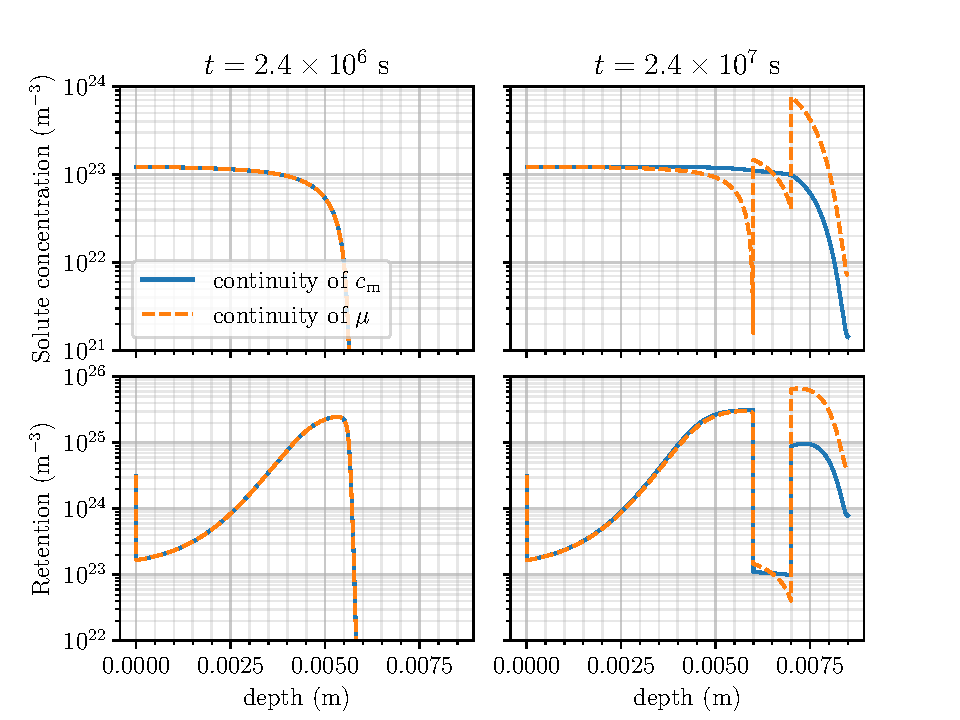
\includegraphics[width=\linewidth]{Figures/Chapter3/monoblocks/interface_condition/iter case/comparison_profiles.pdf}
%     \caption{Comparison of concentrations profiles at several times}
%     \label{fig: concentrations profiles 1D}
% \end{figure}


The steady-state temperature field exhibits high temperature gradients between the plasma-facing surface and the cooling surface (see Figure \ref{fig: temperature}).

\begin{figure}
    \centering
    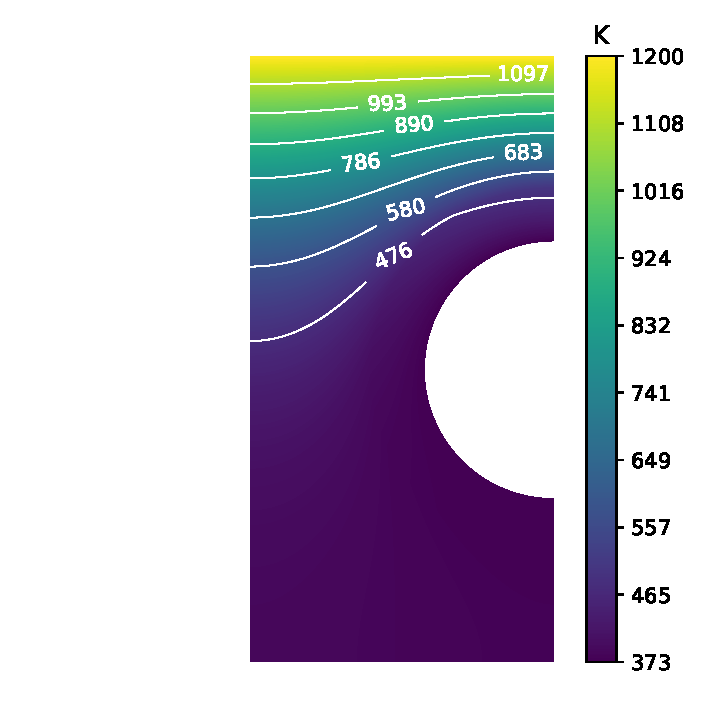
\includegraphics[width=0.8\linewidth]{Figures/Chapter3/monoblocks/interface_condition/iter case/temperature_field_2d.pdf}
    \caption{Steady-state temperature field of an ITER-like monoblock simulated with FESTIM.}
    \label{fig: temperature}
\end{figure}

\begin{figure}
    \centering
    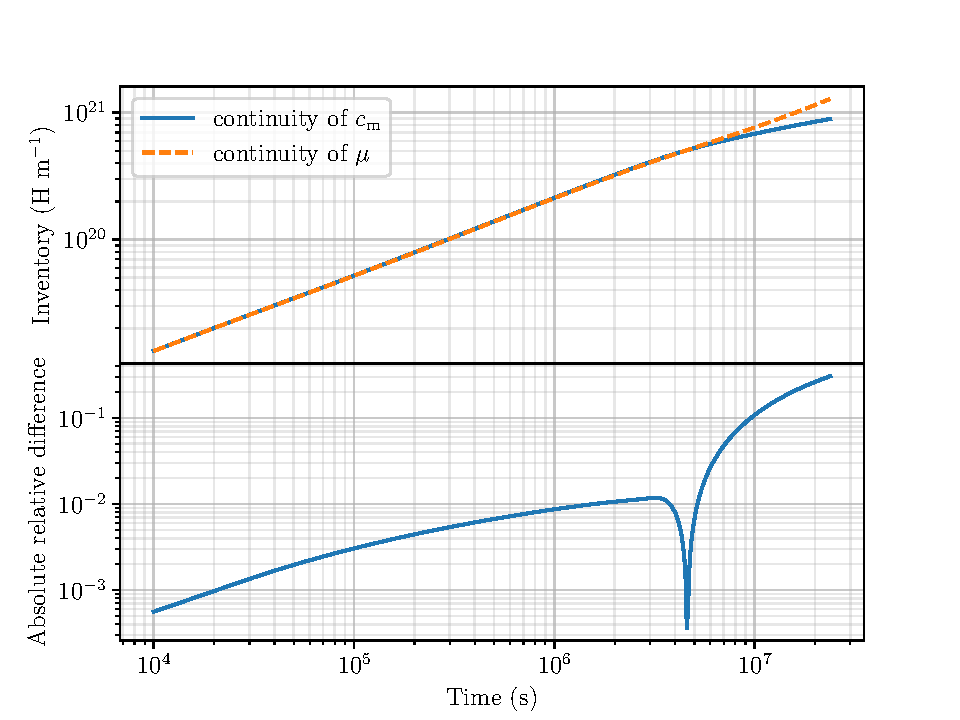
\includegraphics[width=\linewidth]{Figures/Chapter3/monoblocks/interface_condition/iter case/comparison_inventory_2d.pdf}
    \caption{Influence of chemical potential conservation on hydrogen inventory.}
    \label{fig: 2D inventories}
\end{figure}


\begin{figure}
    \centering
    \begin{subfigure}{0.5\linewidth}
        \centering
        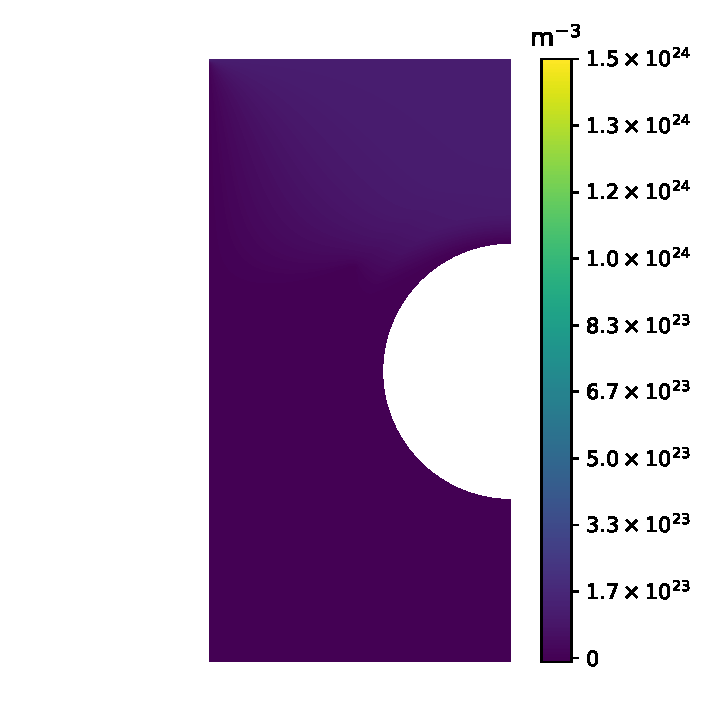
\includegraphics[width=\linewidth]{Figures/Chapter3/monoblocks/interface_condition/iter case/solute_c.pdf}
        \caption{$c_\mathrm{m}$ (continuity of $c_\mathrm{m}$)}
    \end{subfigure}%
    \begin{subfigure}{0.5\linewidth}
        \centering
        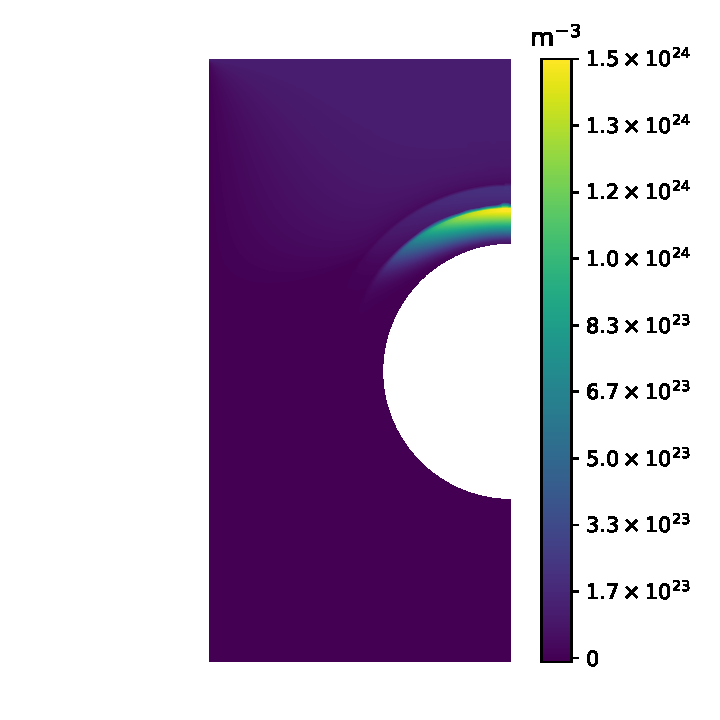
\includegraphics[width=\linewidth]{Figures/Chapter3/monoblocks/interface_condition/iter case/solute_mu.pdf}
        \caption{$c_\mathrm{m}$ (continuity of $\mu$)}
    \end{subfigure}
    \begin{subfigure}{0.5\linewidth}
        \centering
        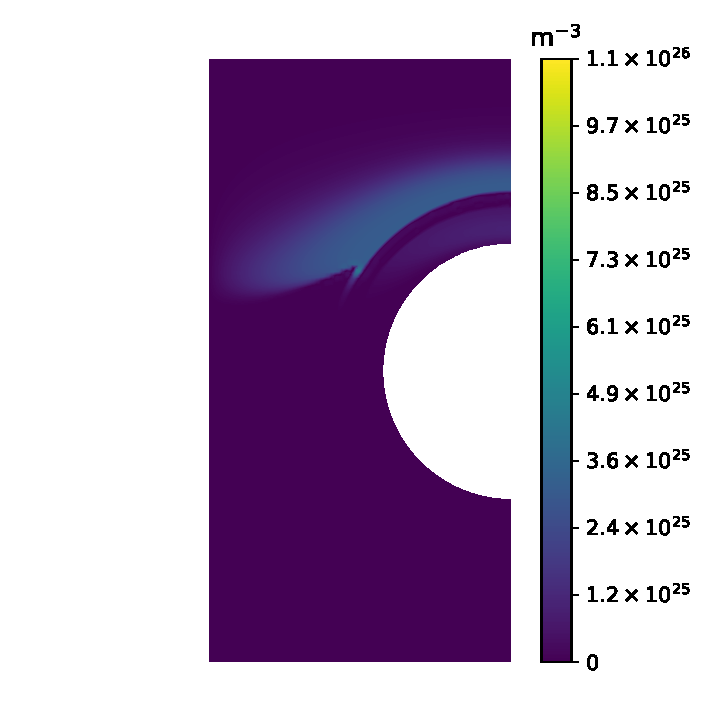
\includegraphics[width=\linewidth]{Figures/Chapter3/monoblocks/interface_condition/iter case/retention_c.pdf}
        \caption{Retention (continuity of $c_\mathrm{m}$)}
    \end{subfigure}%
    \begin{subfigure}{0.5\linewidth}
        \centering
        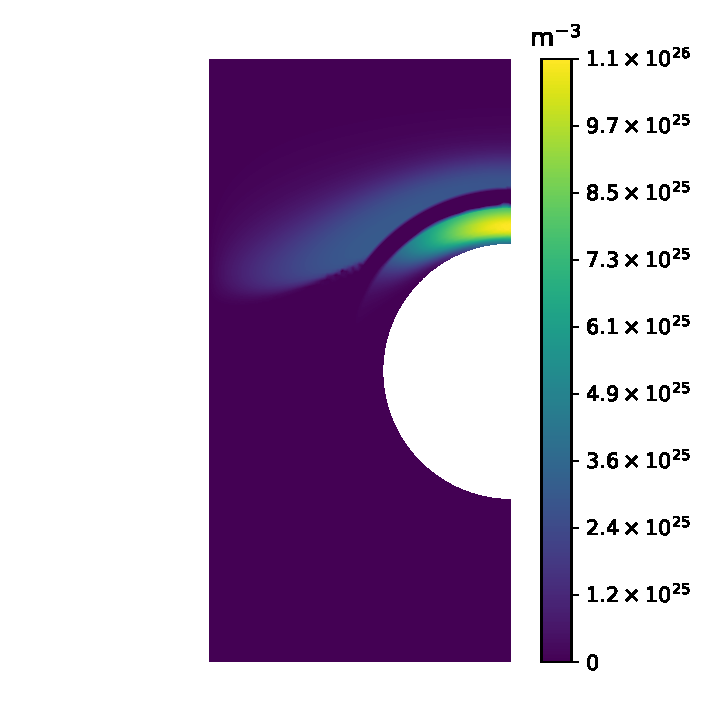
\includegraphics[width=\linewidth]{Figures/Chapter3/monoblocks/interface_condition/iter case/retention_mu.pdf}
        \caption{Retention (continuity of $\mu$)}
    \end{subfigure}
    \caption{2D concentration fields at $t=\SI{2.4e7}{s}$}
    \label{fig: concentrations fields 2d}
\end{figure}
Two cases were examined, one with mobile concentration $c_\mathrm{m}$ continuity at interfaces and the other with continuity of chemical potential (\textit{ie.} continuity of $c_\mathrm{m}/S$).

Up to \SI{5e6}{s}, there was no difference in the total hydrogen inventory between the two cases (see Figure \ref{fig: 2D inventories}).
It is only after this implantation that the inventory of the two cases started to diverge.
At $t=\SI{2.4e7}{s}$, the inventory of the continuity of chemical potential case was higher than with continuity of $c_\mathrm{m}$.
This is explained by the high solubility ratio between Cu and CuCrZr leading to a higher concentration of mobile particles in CuCrZr and therefore a higher trapping rate.
However, even then, the trap density in Cu being low compared to other materials, the global inventory is not affected much.
For these two reasons, the inventories are unaffected before \SI{5e6}{s}.

Similarily, before reaching the W/Cu interface, the $c_\mathrm{m}$ and retention profiles are identical regardless of the interface condition (see Figure \ref{fig: concentrations fields 2d}).
Once the W/Cu interface is reached, the $c_\mathrm{m}$ profiles are affected by the interface condition.
The interface condition had no influence whatsoever on the mobile particle concentration $c_\mathrm{m}$ in the W.
However, $c_\mathrm{m}$ was higher in Cu and CuCrZr in the case with chemical potential conservation (up to \SI{1.5e24}{m^{-3}} in CuCrZr at $t=\SI{2.4e7}{s}$).
This increase of $c_\mathrm{m}$ leads to an increase of the trap occupancy and therefore an increase of the local retention.

The retro-desorbed flux (from the monoblock to the plasma) does not depend on the interface conditions since interfaces are far from the exposed surface.
Moreover, outgassing flux through the cooling pipe greatly depends on the boundary condition imposed at the cooling surface.
Therefore, in order to assess the impact of interface conditions on the outgassing flux through the cooling pipe, uncertainties must first be lift regarding the recombination process occurring on surfaces in contact with water.

% \subsection{Summary}
% should we keep this
% The influence of interface conditions between materials has been studied with FESTIM.
% A novel approach has been implemented in FESTIM in order to ensure equilibrium at the interfaces.
% The implementation has been verified using the Method of Exact Solutions and the Method of Manufactured Solutions.
% % A comparison test has been performed with TMAP7 and Abaqus and the three codes show very good agreement.

% H transport through Cu/EUROFER and W/Cu composite slabs has been studied.
% It is shown that the interface condition can have an impact on the outgassing flux.
% This modelling work will help design future permeation barriers in DEMO.
% A method for identifying material properties with either an analytical solution or with the FESTIM code is also described.

% The influence of interface conditions is also studied on the ITER monoblock test case in both 1D and 2D.
% It is shown that this has very low influence up to \SI{5e6}{s} and that discrepancies only start to appear after a very long exposure time.
% This is because interfaces are far from the exposed surface and hydrogen atoms only reach these interface after a long exposure time.
% The continuity of mobile concentration can therefore be employed safely for monoblocks H transport simulations in order to assess monoblocks inventory.
% This is especially true when desorption is assumed on the edges of the monoblock where less H particles will reach the interfaces.
% In other words, the effect of the interfaces conditions is negligible compared to the edge effects (this will be shown in more details in Section \ref{3D edge effects}).
